\documentclass{article}
\usepackage{graphicx}
\usepackage{amsmath}
\usepackage{float}
\usepackage{amsfonts}
\usepackage{listings}
\usepackage{xcolor}
\usepackage[utf8]{inputenc}
\usepackage{hyperref}
\usepackage{fancybox}
\usepackage{booktabs}
\usepackage{array}
\usepackage{tikz}
\usepackage{dsfont}
\usepackage{pgfplots}
\pgfplotsset{compat=1.18}
\usepackage[margin=2cm]{geometry}
\usepackage[french]{babel} % Pour les éléments en français
\usetikzlibrary{shapes, arrows.meta, positioning}
\usepackage[labelfont=bf, font=small]{caption}  % Pour personnaliser le titre de la figure


\title{HAX711X - Analyse des Données Multidimensionnelles \\ DM2 Classification automatique}
\author{SCAIA Matteo et MARIAC Damien}
\date{\today} 

\begin{document}

\maketitle

\begin{figure}[h] 
    \centering
    
\includegraphics[width=0.5\textwidth]{ssd_logo.png} 
\end{figure}

\begin{figure}[h] 
    \centering
    
\includegraphics[width=0.5\textwidth]{logo_um_2022_rouge_RVB.png} 
\end{figure}

\newpage

\tableofcontents

\newpage
\section{Treillis de Galois}
\subsection{Création du treillis}
Dans cette question, nous allons analyser le treillis de Galois construit à partir des données fournies par le sujet afin de modéliser les relations entre les films et leurs caractéristiques.
\begin{figure}[h]
    \centering
    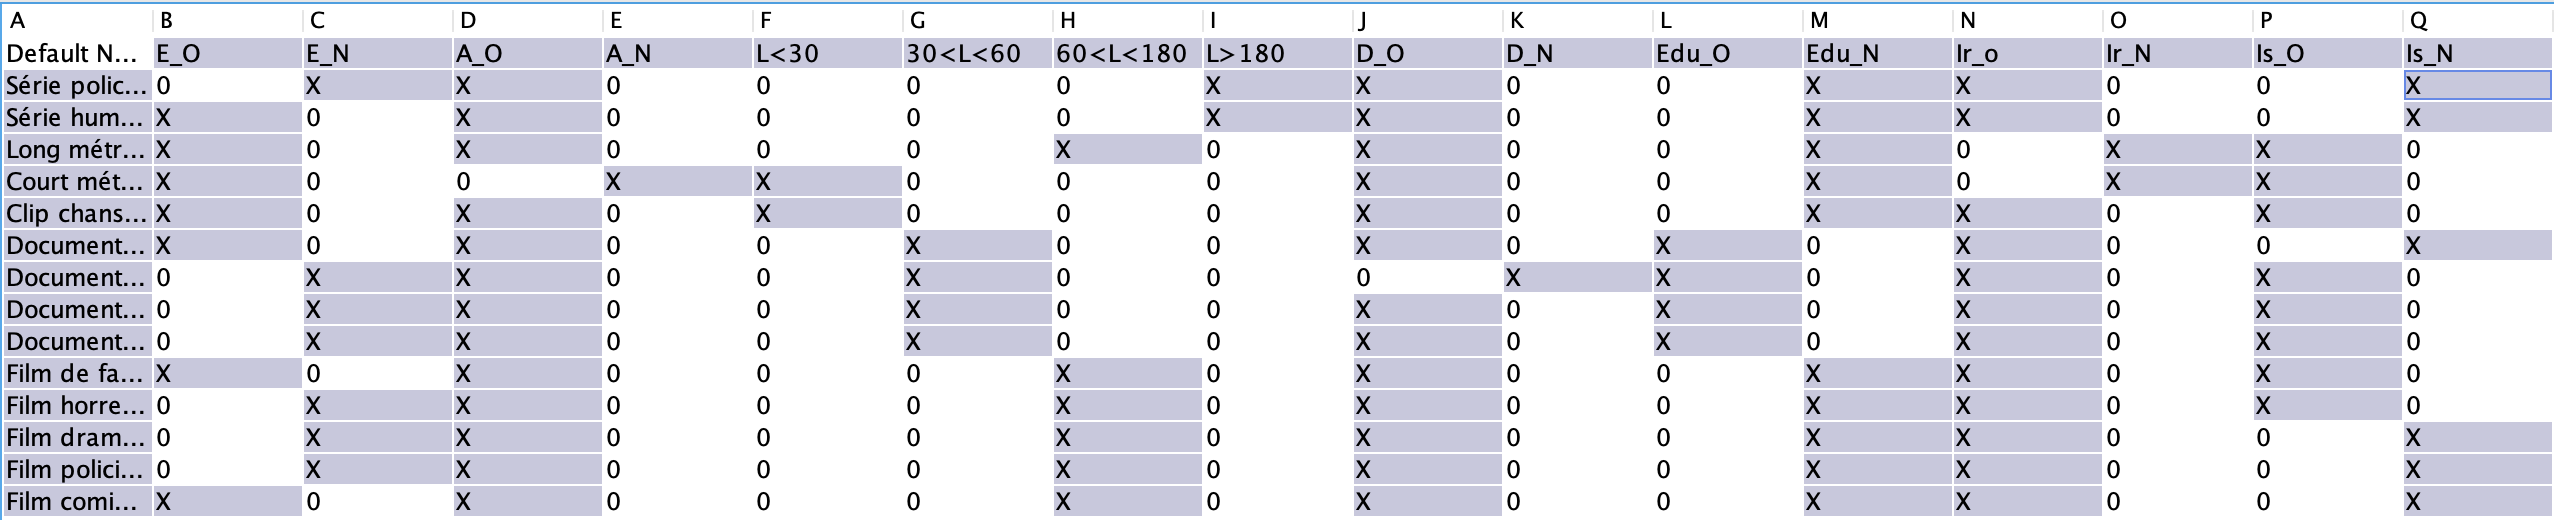
\includegraphics[width=0.7\textwidth]{tableau.png}
    \caption{Tableau des relations binaires}
    \label{fig:tableau} 
\end{figure}
\\
À l'aide du logiciel Galicia, nous obtenons le treillis de Galois suivant :
\begin{figure}[h]
    \centering
    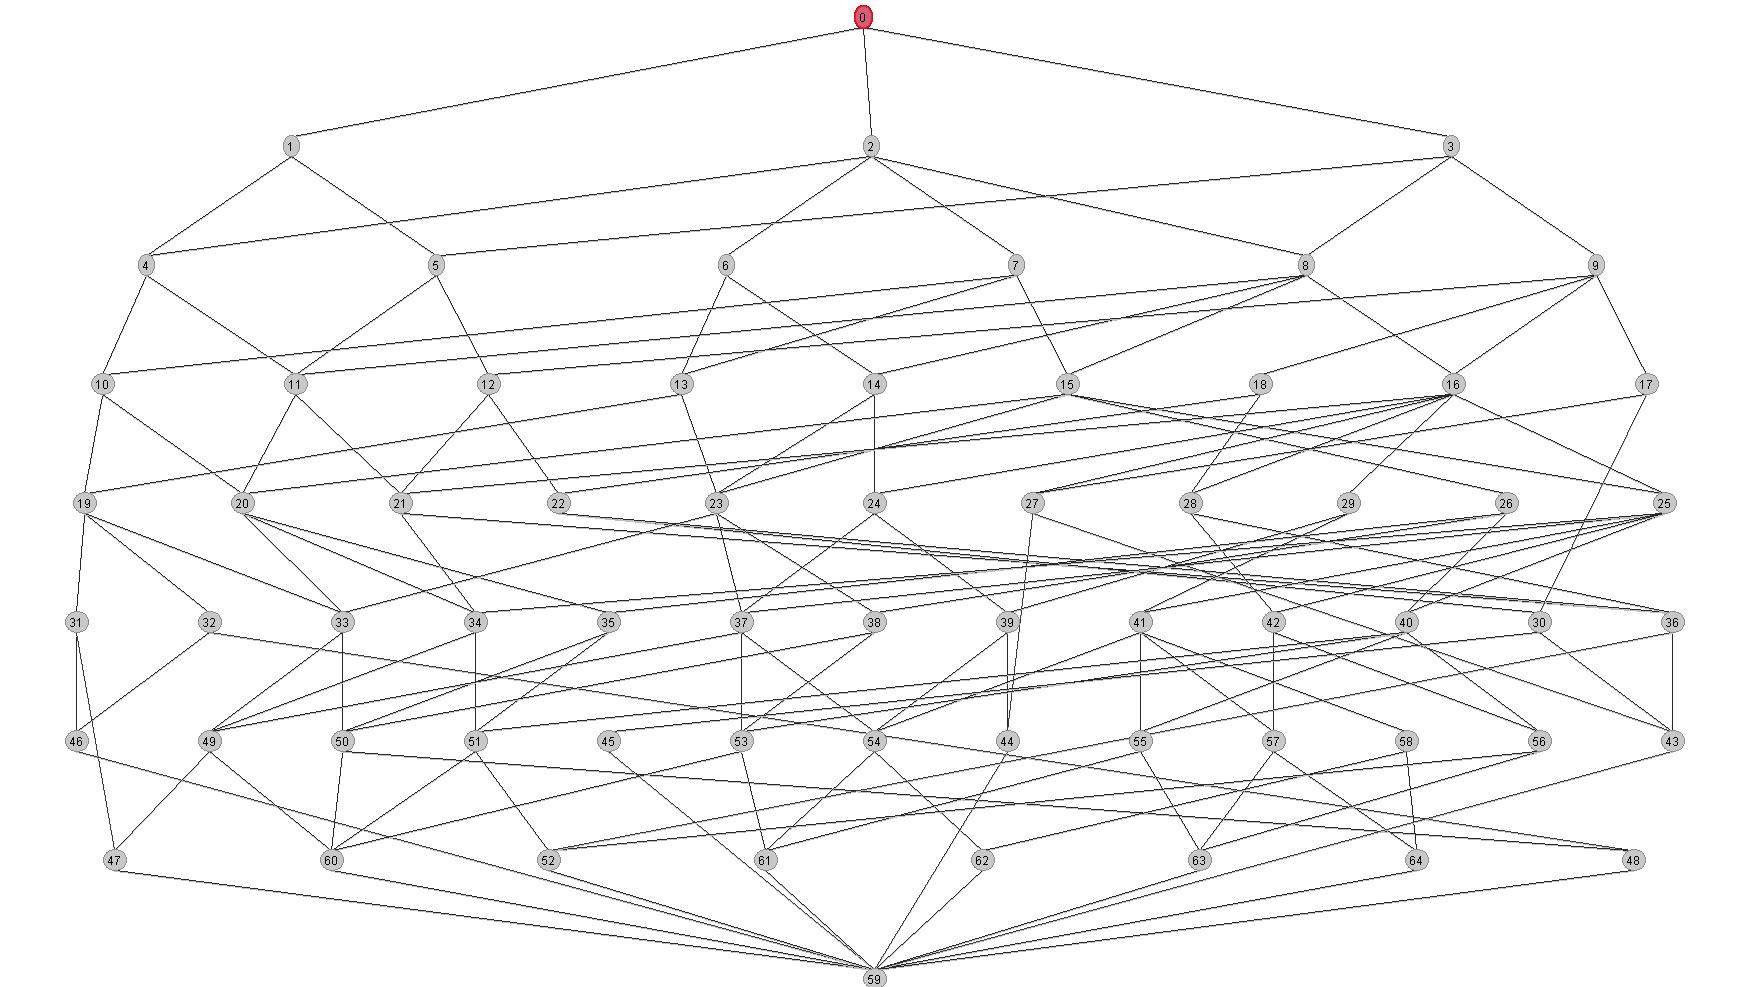
\includegraphics[width=0.7\textwidth]{treillis.png}
    \caption{Treillis de Galois}
    \label{fig:treillis} 
\end{figure}
\\
\subsection{Interprétation}

Dans un treillis de Galois, les nœuds situés aux extrémités correspondent soit à l’ensemble de tous les individus (en haut), soit à l’ensemble de toutes les caractéristiques (en bas). Ces nœuds étant trop généraux ou trop spécifiques, leur analyse n’est pas nécessaire.
\\
\\
Le nœud 57 regroupe les films dramatiques (FD), les films policiers (FP) et les séries policières (SP), caractérisés par les propriétés suivantes : ils s’adressent aux adolescents et aux adultes (A = Oui), ont un objectif distractif (D = Oui), ne sont pas éducatifs (ED = Non), ne ciblent pas les enfants (E = Non), utilisent des images réelles (IR = Oui) et n’incluent pas d’images de synthèse (IS = Non). Ce regroupement correspond à des œuvres qui partagent des thématiques et des intentions narratives du genre "thriller".
\\
Par ailleurs, ce nœud est lié à la classe 42, qui partage les mêmes caractéristiques mais inclut également des œuvres utilisant des images de synthèse. Cela permet d’y intégrer des films d’horreur (FH).
\\
Cette classe peut être interprétée comme un regroupement de film conçues pour provoquer du suspense ou des "frissons".
\\
\\
Le nœud 16 représente une classe large regroupant plusieurs types de films et séries partageant diverses caractéristiques : un public adulte, une vocation distractive, et des images réelles. Ce nœud est particulièrement intéressant, car il se connecte à plusieurs autres classes. Ces caractéristiques sont partagées par des genres variés. De ce fait, cette classe regroupe de nombreux types de films et séries, tels que les clips musicaux, les documentaires artistiques, les documentaires sur la nature, les documentaires scientifiques, les films comiques, les films dramatiques, les films de fantasy, les films d’horreur, ainsi que les séries humoristiques et policières.
\\
\\
On remarque également le nœud 17, qui regroupe tous les documentaires. Les caractéristiques de cette classe sont qu’elle s’adresse aux adultes (A = Oui), a une vocation éducative (ED = Oui), utilise des images réelles (IR = Oui) et correspond à des productions de courte durée (30-60 minutes). Ces caractéristiques décrivent ce que sont les documentaires.
\\



\section{Classification hiérarchique de parcelles forestières tropicales}
Charger dans le logiciel les données relatives au peuplement arboré de la forêt du bassin du Congo
(Datagenus.csv). Inspectez le fichier et corrigez-en les erreurs triviales s'il en est. Ces données fournissent
sur 1000 parcelles de cette forêt: les variables de comptage de 27 espèces d'arbres (gen1, ..., gen27), la
surface de la parcelle, le type forestier (forest) tel qu'identifié par les écologues . On ne tiendra pas compte
des autres variables. Calculer la densité de peuplement de chaque espèce par unité de surface pour les 1000
parcelles. Les parcelles seront traduits en nuage dans l'espace des 27 densités de peuplement.

\subsection{Préparation des données}
\label{Q1}
Nous traduisons les observations dans l’espace euclidien, où la distance servira de mesure de dissimilarité globale entre les parcelles. Cette mesure repose sur la comparaison des écarts sur les différentes dimensions (densités des espèces). Puisque toutes les dimensions (espèces) sont supposées avoir une importance équivalente, aucune ne doit dominer le calcul.
\\
On note $x_i$ la $i$-ième parcelle. La distance euclidienne entre deux parcelles $x_1$ et $x_2$ est :  
\[
d(x_1, x_2) = \sqrt{\sum_{j=1}^{27} (x_1^j - x_2^j)^2}
\]
où \( x_1^j \) et \( x_2^j \) représentent respectivement la densité de l'espèce j dans les parcelles 1 et 2.
\\
En analysant la contribution de chaque espèce, nous obtenons le tableau suivant :
\begin{table}[h!]
    \centering
    \caption{Contribution des espèces (gen1 à gen11)}
    \label{tab:pourcentage}
    \begin{tabular}{@{}l*{11}{c}@{}}
    \toprule
     & gen1 & gen2 & gen3 & gen4 & gen5 & gen6 & gen7 & gen8 & gen9 & gen10 & gen11 \\ 
    \midrule
    Pourcentage & 
    0.23 & 0.00 & 0.03 & 0.00 & 0.01 & 0.05 & 0.00 & 64.90 & 0.07 & 0.48 & 1.03 \\ 
    \bottomrule
    \end{tabular}
    \end{table}
\\
Nous voyons que les variables ne contribuent pas tous de la même manière. Les contributions des espèces gen1 à gen27 à la distance euclidienne ne sont pas uniformes. Par exemple, gen8 représente 64.90 \% de la distance, ce qui montre que les variations dans cette dimension dominent les calculs de dissimilarité.
\\
Nous standardisons les densités de peuplement et on note \( \mathbf{Z} \) la matrice associée :

\[
z_i^j = \frac{x_i^j - \overline{x}^j}{\sigma_{x^j}}
\]
avec \( x_i^j \) la densité de l’espèce \( j \) sur la parcelle \( i \), \( \overline{x}^j \) la moyenne des densités pour l’espèce \( j \), et \( \sigma_{x^j} \) l’écart-type de l’espèce \( j \).\\
La standardisation assure que chaque dimension contribue de manière équivalente à la mesure de la dissimilarité, indépendamment de son échelle initiale ou de sa variabilité.
\subsection{CAH des parcelles sur les densités de peuplement}
\subsubsection{Classification ascendante hiérarchique}
Dans cette section, nous procéderons à la classification des parcelles en fonction de leur peuplement arboré. L'objectif est de déterminer le nombre optimal de classes pertinentes pour cette partition. À partir des données standardisées représentant les densités de peuplement obtenues à la question \ref{Q1}, nous utiliserons le code en langage R fourni dans le sujet pour effectuer une classification ascendante hiérarchique (CAH). Cette méthode nous permettra d’identifier les classes les plus adaptées à la caractérisation des parcelles.
Nous allons utiliser divers indice d'agrégation (Ward, maximum, moyen) qui permettent de mesurer la difficulté d'agrégation de deux classes.
L'indice de saut minimum étant à part nous ne l'utiliserons pas. En effet, ses résultats sont trop différents. Il permet de dépister les chaines/continuité.
\\
\\
\textbullet\ \underline{Indice de Ward}
\\
L'indice de Ward est définie par :
\\
\\
Soient A et B deux classes de centre de gravité $\bar{x}_A$ et $\bar{x}_B$, et de poids $w_A$ et $w_B$.
\[
\mu_\text{Ward} (A,B) = \frac{w_A w_B}{w_A + w_B} \left\lVert \bar{x}_B - \bar{x}_A \right\lVert ^2
\]
\\
Avec cette indice, nous obtenons le dendogramme suivant :
\\
\begin{figure}[H]
    \centering
    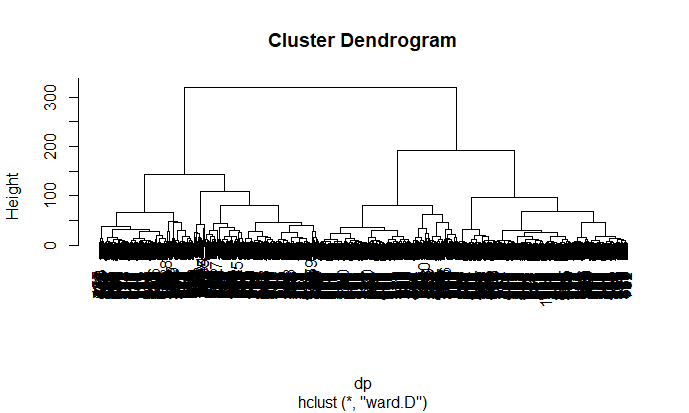
\includegraphics[width=0.8\textwidth]{WARDDENDO.png}
    \caption{Dendogramme (indice de Ward)}
    \label{fig:Ward} 
\end{figure}
On remarque que l'on peut partitionner notre arbre en 4 classes.
Pour confirmer notre choix d’utiliser 4 classes, nous pouvons utiliser l’histogramme des niveaux de $\mu_{ward}$.
\begin{figure}[H]
    \centering
    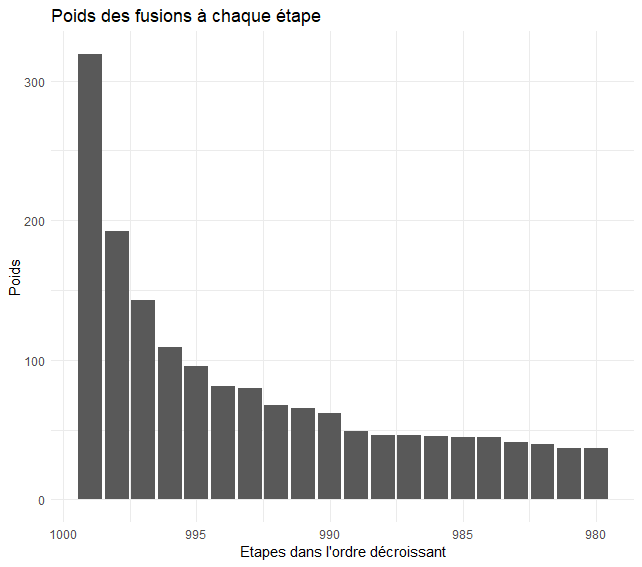
\includegraphics[width=0.3\textwidth]{histoward.png}
    \caption{Histogramme des niveaux $\mu_{Ward}$}
    \label{fig:HWard} 
\end{figure}

La figure \ref{fig:HWard} illustre que la différence de coût d'agrégation entre une partition en quatre classes et une partition en cinq classes est relativement faible. Par conséquent, une partition en quatre classes semble appropriée. 

Les \( R^2 \) associés à chaque classe sont ensuite calculés :

\begin{figure}[H]
    \centering
    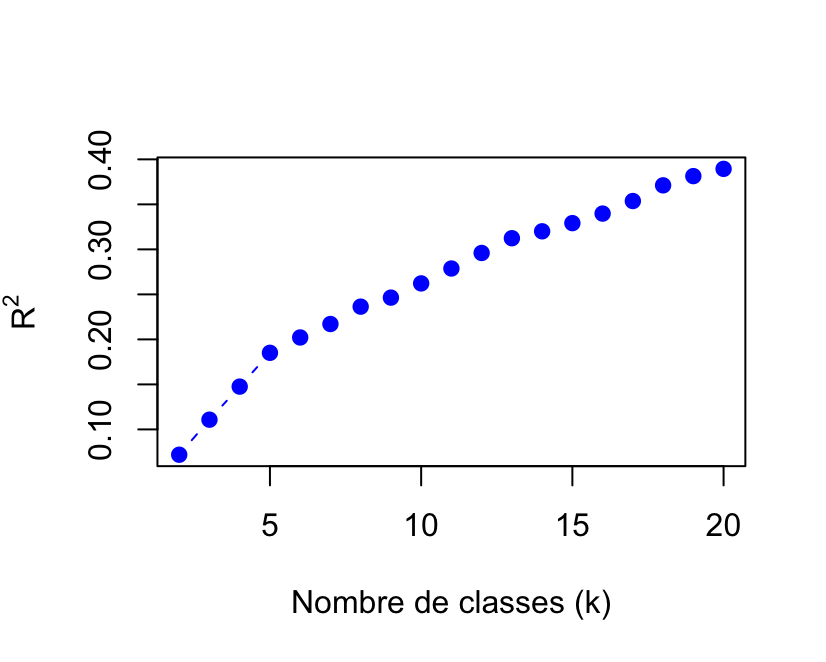
\includegraphics[width=0.5\textwidth]{R222.png}
    \caption{Evolution du R2 en fonction du nombre de classe}
    \label{fig:EvolR2} 
\end{figure}
À partir de ce graphique, nous constatons que les partitions potentielles sont en 3, 4 et 5 classes, avec des \( R^2 \) respectifs de 0.111, 0.148 et 0.185. Nous décidons donc d'opter pour une partition en 4 classes.
\\
Ainsi, nous obtenons la répartition suivante :
\begin{figure}[H]
    \centering
    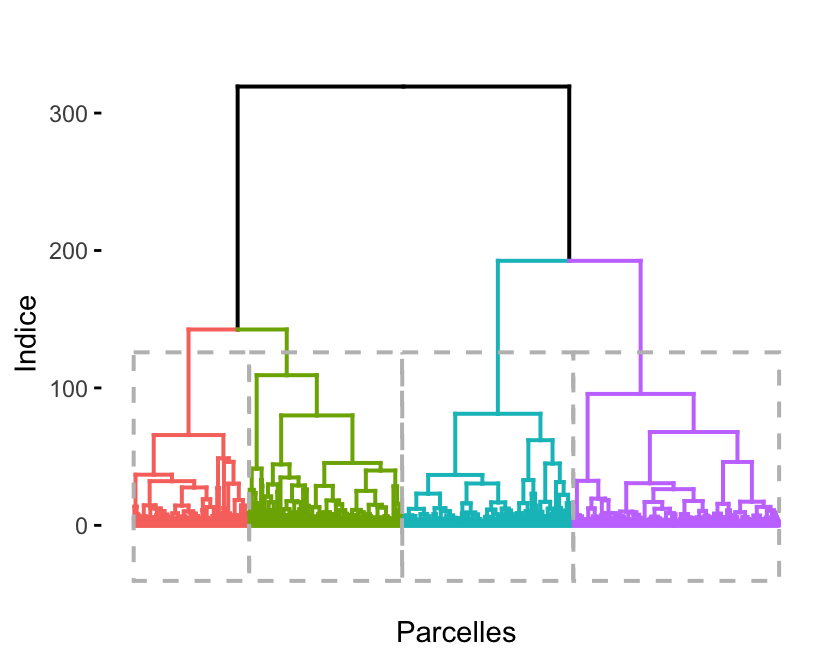
\includegraphics[width=0.5\textwidth]{wardcouleur.png}
    \caption{Dendogramme indice de Ward}
    \label{fig:Ward_couleur} 
\end{figure}

\textbullet\ \underline{Indice du saut maximum}
\\
La méthode du saut maximum consiste à mesurer la similitude avec la paire la plus eloignée
L'indice de saut maximum est définie par :
\\
\\
Soient A et B deux classes :
\[
\mu(A,B) = \max_{a \in A , b \in B} d(a,b)
\]
\\
Avec l'indice de saut maximum, on obtient le dendogramme suivant:
\\
\begin{figure}[H]
    \centering
    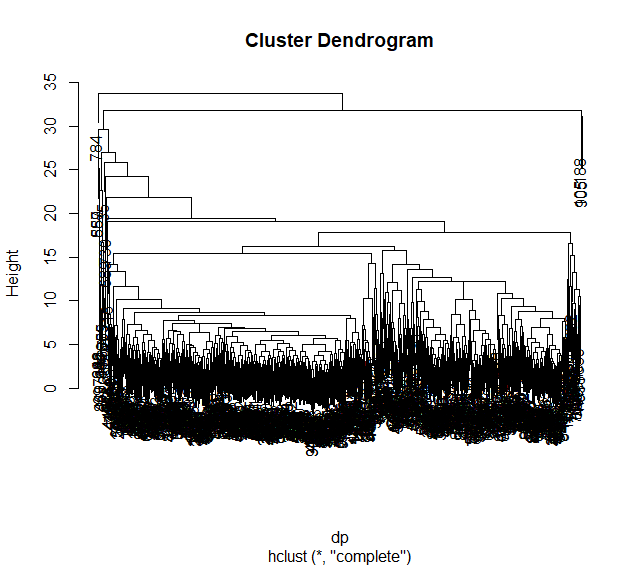
\includegraphics[width=0.5\textwidth]{dendromax4.png}
    \caption{Dendrogramme  indice du saut max}
    \label{fig:dendmax} 
\end{figure}
Avec son histogramme associé
\\
\begin{figure}[H]
    \centering
    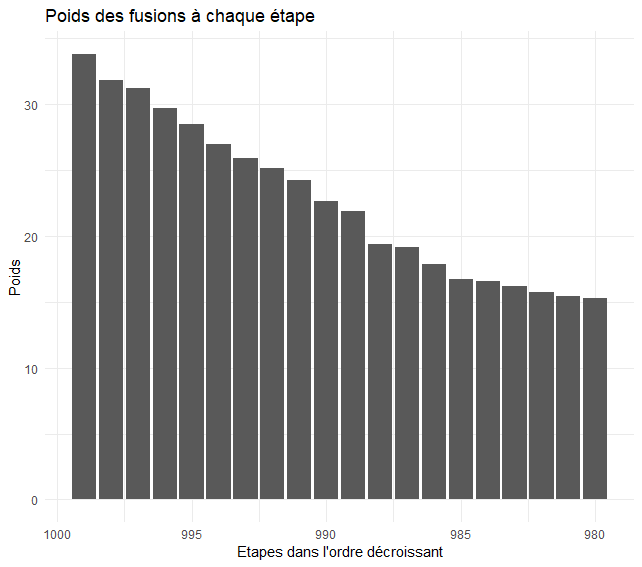
\includegraphics[width=0.3\textwidth]{histomax4.png}
    \caption{Histogramme des niveaux saut maximum}
    \label{fig:histomax} 
\end{figure}
L'examen de la figure \ref{fig:dendmax} révèle la présence de points atypiques, notamment les parcelles 905, 105 et 188, qui se distinguent par leur position en haut à droite du graphique. L'interprétation du nombre optimal de classes à partir de cette figure s'avère délicate. Afin de clarifier cette question, nous avons tracé l'histogramme présenté en figure \ref{fig:histomax}. Celui-ci permet de constater qu'un partitionnement en quatre classes semble le plus pertinent pour notre analyse.
\\\\

\textbullet\ \underline{Comparaison}
\\\\
Pour évaluer le degré de similarité entre deux partitions \( P \) et \( P' \), nous utilisons l'indice de Rand. Cette mesure repose sur l'examen de toutes les paires d'éléments présentes dans les partitions.
\\
Nous obtenons les résultats suivant :
\begin{table}[ht]
    \centering
    \begin{tabular}{|c|c|}
    \hline
    \textbf{Comparaison des partitions} & \textbf{Indice de Rand} \\
    \hline
    \( P_{\text{WARD}} \) et \( P_{\text{MAX}} \) & 0.2639 \\
    \( P_{\text{WARD}} \) et \( P_{\text{MOYEN}} \) & 0.2629 \\
    \( P_{\text{MAX}} \) et \( P_{\text{MOYEN}} \) & 0.9980 \\
    \( P_{\text{MIN}} \) et \( P_{\text{MOYEN}} \) & 0.9960 \\
    \hline
    \end{tabular}
    \caption{Comparaison des partitions à l'aide de l'indice de Rand}
    \end{table}
\\
Les indices de Rand montrent que les partitions obtenues par les méthodes \textit{Ward} et \textit{Max} (0.2639), ainsi que \textit{Ward} et \textit{Moyen} (0.2629), sont relativement peu similaires, indiquant des différences notables dans le regroupement des éléments. En revanche, les partitions \textit{Max} et \textit{Moyen} (0.9980) ainsi que \textit{Min} et \textit{Moyen} (0.9960) sont presque identiques, suggérant une forte similarité dans les regroupements effectués par ces méthodes. Ainsi, les partitions \textit{Max}, \textit{Min}, et \textit{Moyen} se ressemblent beaucoup, tandis que \textit{Ward} produit une partition distincte.



\subsection{Optimisation d'une partition avec les K-means}
Après avoir identifié une partition en 4 classes prometteuse avec la CAH. Nous poursuivons l'analyse en optimisant ces groupements à l'aide de la méthode des K-means. 
La commande kmeans de R nous permet de calculer une partition à partir d'un jeu de 
données et de centres de gravité. Montrons que les centres de gravité sont bien obtenus par la formule que nous avons implementée.

Avec les notations du cours, nous savons que les centres de gravités correspondent aux moyennes par classes de chaque variable. Ainsi, nous pouvons utiliser la formule démontrée en cours.
\par\textbf{Notons :}
\begin{itemize}
    \item $X \in \mathbb{R}^{1000\times 27}$ la matrice des variables quantitatives.
    \item $M \in \mathbb{R}^{1000\times 4}$ la matrice indicatrice des modalités.
    \item $W = \frac{1}{1000} I_{1000}$ la matrice des poids des individus.
    \item $C \in \mathbb{R}^{4\times 27}$ la matrice des centres de gravité.
\end{itemize}

On a alors, 

\begin{align*}
    C &= (M'WM)^{-1}M'WX = (M'\frac{1}{1000} I_{1000} M)^{-1}M' \frac{1}{1000} I_{1000} X \\
    &=\frac{1000}{1000}(M'M)^{-1} M'X \\
    &= (M'M)^{-1} M'X
\end{align*}
Ce que l'on voulait démontrer.
\\
\\
Après l'implémentation de la méthode des K-means, nous observons une valeur de $R^2=0.180$ Cette valeur indique une amélioration de la partition des classes.

\begin{center}
    \begin{minipage}{0.45\textwidth}
        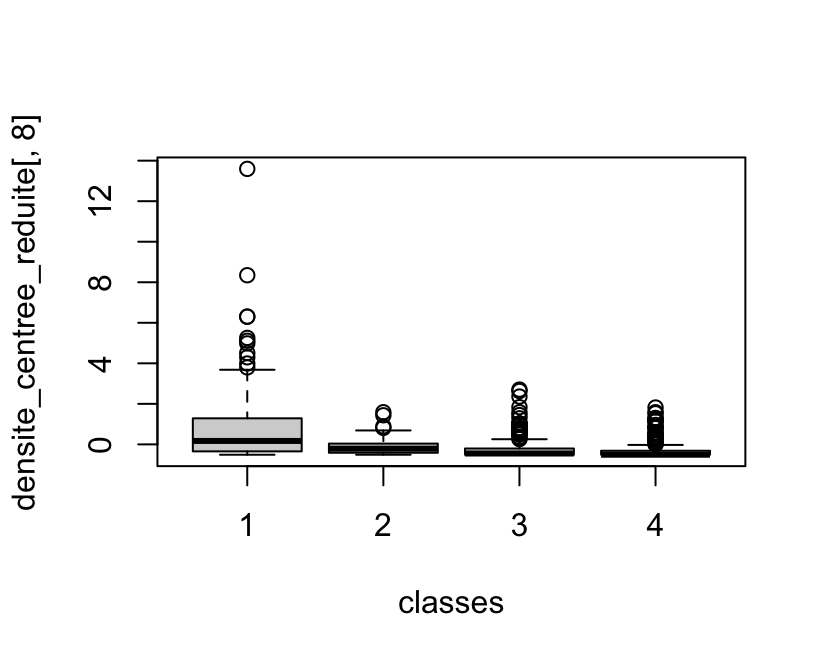
\includegraphics[width=\textwidth]{avant kkkkk.png}
        \captionof{figure}{Boites à moustache pour l'espèce 10 avant K-means }
    \end{minipage}
    \hfill
    \begin{minipage}{0.45\textwidth}
        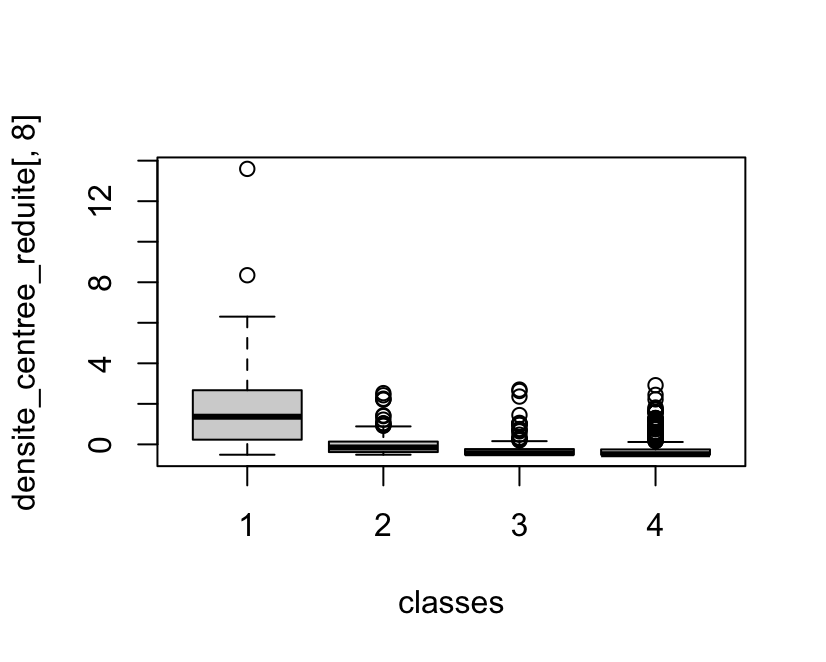
\includegraphics[width=\textwidth]{apres kkkkk.png}
        \captionof{figure}{Boites à moustache pour l'espèce 10 après K-means }
    \end{minipage}
\end{center}
À partir des deux figures précédentes, nous observons un des effets de la méthode des K-means. La différence la plus marquante concerne la classe 1, où l'on constate une diminution des valeurs atypiques et un changement de la médiane.\\
Nous souhaitons désormais interpréter les classes obtenues. À cet effet, nous utiliserons l'indice de Tschuprow pour examiner l'association entre les variables, à savoir le type forestier et le type géologique, avec les classes formées.
Nous rappelons que l'indice de Tshuprow est donné par : 
\[
T^2 = \frac{\phi^2 (X,Y)}{\sqrt{I-1}\sqrt{J-1}} 
\]
avec I le nombre de modalité de X une variable nominale et J le nombre de modalité de Y une variable nominale et $\phi^2$ le coefficient de contingence qui mesure la liaison entre deux variables. 
\\
Nous obtenons alors, pour le type forestier, une valeur de $0.325$, et pour le type géologique, une valeur de $0.369$.  
Bien que l'indice ne révèle pas une forte association, il montre tout de même une certaine relation entre le type forestier et les classes.

Nous analysons la distribution des types forestiers et géologiques au sein de chaque classe dans le but d'extraire des informations pertinentes.

\newpage
\begin{table}[H]
    \centering
    \begin{minipage}{0.48\textwidth} % Commence un minipage pour le premier tableau
        \centering
        \begin{tabular}{|l|l|l|l|l|}
        \hline
                            & 1     & 2     & 3     & 4     \\ \hline
        1                   & 0.500 & 0.167 & 0.432 & 0.208 \\ \hline
        2                   & 0.106 & 0.008 & 0.054 & 0.190 \\ \hline
        3                   & 0.058 & 0.004 & 0.014 & 0.028 \\ \hline
        4                   & 0.086 & 0     & 0.027 & 0.007 \\ \hline
        5                   & 0.144 & 0.047 & 0.140 & 0.263 \\ \hline
        6                   & 0.058 & 0.024 & 0.086 & 0.152 \\ \hline
        7                   & 0.048 & 0.750 & 0.248 & 0.151 \\ \hline
        \end{tabular}
        \caption{Proportion type forestier}
    \end{minipage}\hfill % Fin du premier minipage et ajout d'un espace entre les deux
    \begin{minipage}{0.48\textwidth} % Commence un minipage pour le second tableau
        \centering

        \begin{tabular}{|l|l|l|l|l|}
        \hline
                            & 1     & 2     & 3     & 4     \\ \hline
        1                   & 0.038 & 0.019 & 0.158 & 0.145 \\ \hline
        2                   & 0.087 & 0.004 & 0.131 & 0.052 \\ \hline
        3                   & 0.240 & 0.758 & 0.018 & 0.161 \\ \hline
        5                   & 0.221 & 0.012 & 0.423 & 0.191 \\ \hline
        6                   & 0.413 & 0.206 & 0.270 & 0.450 \\ \hline
        \end{tabular}
        \caption{Proportion type geologique}
    \end{minipage}
\end{table}
(Le type géologique 4 n'est pas présent dans les données de base.)
\\

Globalement, les classes 1 et 4 présentent des similitudes dans leurs caractéristiques géologiques et forestières. Toutefois, elles se distinguent par une prédominance du type géologique 1 dans la classe 4. De plus, elles diffèrent en ce qui concerne la proportion du type forestier 1, qui est plus présente dans la classe 1 que dans la classe 4.
\\
La classe 2 se caractérise par une forte présence du type forestier 7 et du type géologique 3, tandis qu'elle affiche une faible proportion du type forestier 3 et une absence de type forestier 4.
\\
Quant à la classe 3, elle montre une faible proportion du type géologique 3, représentant seulement 1,8~\% de sa composition.
\\
Ces observations mettent en évidence des variations spécifiques dans la distribution des types géologiques et forestiers au sein des différentes classes.


\newpage
\section{ANNEXE}

\end{document}